\begin{figure}
\vspace*{11mm}
\hspace*{73mm}
\begin{tikzpicture}[transform canvas={scale=0.73}]
  \node (A) {
    \begin{tikzpicture}
      \node[inner sep=0pt] (c1) {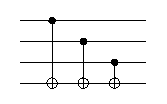
\includegraphics[scale=2]{Figures/circuits/proof1}};  
      \coordinate[below left=7mm and -6mm of c1.west] (l1);
      \coordinate[right=45mm of l1] (r1);
      \pic (cut1) {cut=l1/r1};     
      \node[right=0mm of c1] (eq1) {\Large \(=\)}; 
      \node[right=0mm of eq1, inner sep=0pt] (c2) {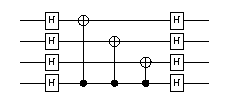
\includegraphics[scale=2]{Figures/circuits/proof2}};  
      \coordinate[below left=7mm and -6mm of c2.west] (l2);
      \coordinate[right=66mm of l2] (r2);
      \pic (cut2) {cut=l2/r2};  
      \node[right=0mm of c2] (eq2) {\Large \(=\)};  
    \end{tikzpicture}
  };
  \node[below=5mm of A] (B) {
    \begin{tikzpicture}
      \node (eq2) {\Large \(=\)};    
      \node[right=-4mm of eq2, inner sep=0pt] (circuit) {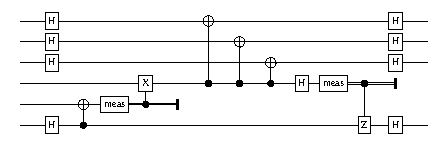
\includegraphics[scale=2]{Figures/circuits/proof3}};  
      \pic (e3) {ebit=e3/26.79mm/13mm};  
      \coordinate[below left=7mm and -6mm of circuit.west] (l3);
      \coordinate[right=140mm of l3] (r3);
      \pic (cut3) {cut=l3/r3};  
      \node[right=0mm of circuit] (eq3) {\Large \(=\)}; 
    \end{tikzpicture}
  };
  \node[below=5mm of B] (C) {
    \begin{tikzpicture}
      \node (eq3) {\Large \(=\)}; 
      \node[right=0mm of eq3, inner sep=0pt] (circuit) {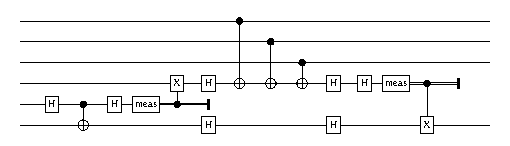
\includegraphics[scale=2]{Figures/circuits/proof4}};   
      \pic (e4) {ebit=e4/26.79mm/13mm};  
      \coordinate[below left=7mm and -6mm of circuit.west] (l4);
      \coordinate[right=161mm of l4] (r4);
      \pic (cut4) {cut=l4/r4};  
      \node[right=0mm of circuit] (eq4) {\Large \(=\)}; 
    \end{tikzpicture}
  };
  \node[below=5mm of C] (D) {
    \begin{tikzpicture}
      \node (eq4) {\Large \(=\)};    
      \node[right=-4mm of eq4, inner sep=0pt] (circuit) {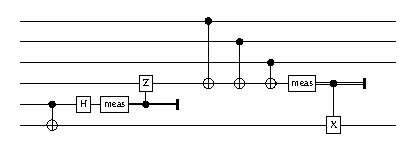
\includegraphics[scale=2]{Figures/circuits/proof5}};     
      \pic (e5) {ebit=e5/26.79mm/13mm};  
      \coordinate[below left=7mm and -6mm of circuit.west] (l5);
      \coordinate[right=129mm of l5] (r5);
      \pic (cut5) {cut=l5/r5};  
      \node[right=-4mm of circuit] (eq5) {\Large \(=\)};    
      \node[right=-4mm of eq5, inner sep=0pt] (c6) {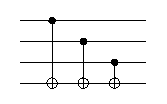
\includegraphics[scale=2]{Figures/circuits/proof1}};   
      \coordinate[below left=7mm and -6mm of c6.west] (l6);
      \coordinate[right=45mm of l6] (r6);
      \pic (cut6) {cut=l6/r6};  
    \end{tikzpicture}
  };
\end{tikzpicture}
\vspace*{140mm}
\caption{Proof of the implementation of multiple non-local CNOT gates that share a common target. The proof uses properties given in Figures~\ref{fig:props}, \ref{fig:sliding} and~\ref{fig:nonlocalCNOTs}. The distributed circuit is similar to the case for share control (Figure~\ref{fig:nonlocalCNOTs}). Both cat-entangler and cat-disentangler slightly differ.}
\label{fig:CNOTtargetProof}
\end{figure}